\chapter{Setup}

% dark box
% power supplies
% multimeter
% osci
% gandalf + clock
% led + diffusor
% emusic
% sipm
\section{SiPM}
An important part of the setup are of course the \acp{sipm} which generate the charge signal which than gets amplified by the \ac{emusic} chips.
The \acp{sipm} mainly used in this work are the \textit{S14160-3050HS} by the manufacturer Hamamatsu.
Another \ac{sipm} model which was used at the \ac{desy} testbeam besides the \textit{S14160-3050HS} is the SensL \textit{J-Series 30035} manufactured by Onsemi.
Some important parameters of both \ac{sipm} models are listed in \autoref{tab:sipm_specs}.
For this work, \acp{pcb} with forty \acp{sipm} soldered onto it were used.
These boards exist with both \ac{sipm} models.
A picture of one of these \acp{pcb} equiped with Hamamatsu \acp{sipm} is shown in \autoref{fig:sipm_pcb}.
A breakout board can be plugged in on the back of the \ac{pcb}.
For this thesis the \ac{emusic} board was used as a breakout board, which is described in the previous chapter.
\begin{table}
	\centering
	\caption[SiPM parameters]{Relevant parameters of the both used \ac{sipm} models by Hamamatsu and Onsemi. \cite{}}
	\label{tab:sipm_specs}
	\renewcommand{\arraystretch}{1.3}
	\begin{tabularx}{\textwidth}{Xp{0.19\textwidth}p{0.15\textwidth}}
	    \toprule
	    parameter								& S14160-3050HS		& SensL			\\\midrule
	    photosensitive are / $\si{\milli\meter\squared}$			& 3.0$\times$3.0	& 3.07$\times$3.07	\\
	    pixel pitch / $\si{\micro\meter}$					& 50			& 35			\\
	    number of pixels							& 3000			& \num{5676}		\\
	    spectral response range / $\si{\nano\meter}$			& \numrange{270}{900}	& \numrange{200}{900}	\\
	    peak sensitivity wavenlength / $\si{\nano\meter}$			& 450			& 420			\\
	    peak photon detection eficiency / $\si{\percent}$			& 50			& 			\\
	    breakdown voltage / $\si{\volt}$					& 38			& \numrange{24.2}{24.7}	\\
	    recommended operating voltage / $\si{\volt}$			& 40.7			& \numrange{25.2}{30.7}	\\
	    variation of rec. op. voltage (typ. / max) / $\si{\volt}$		& 0.1 / 0.2		&			\\
	    gain								& \num{2.5e6}		&			\\
	    \bottomrule
	\end{tabularx}
	\renewcommand{\arraystretch}{1}
\end{table} 
\begin{figure}
	\centering
	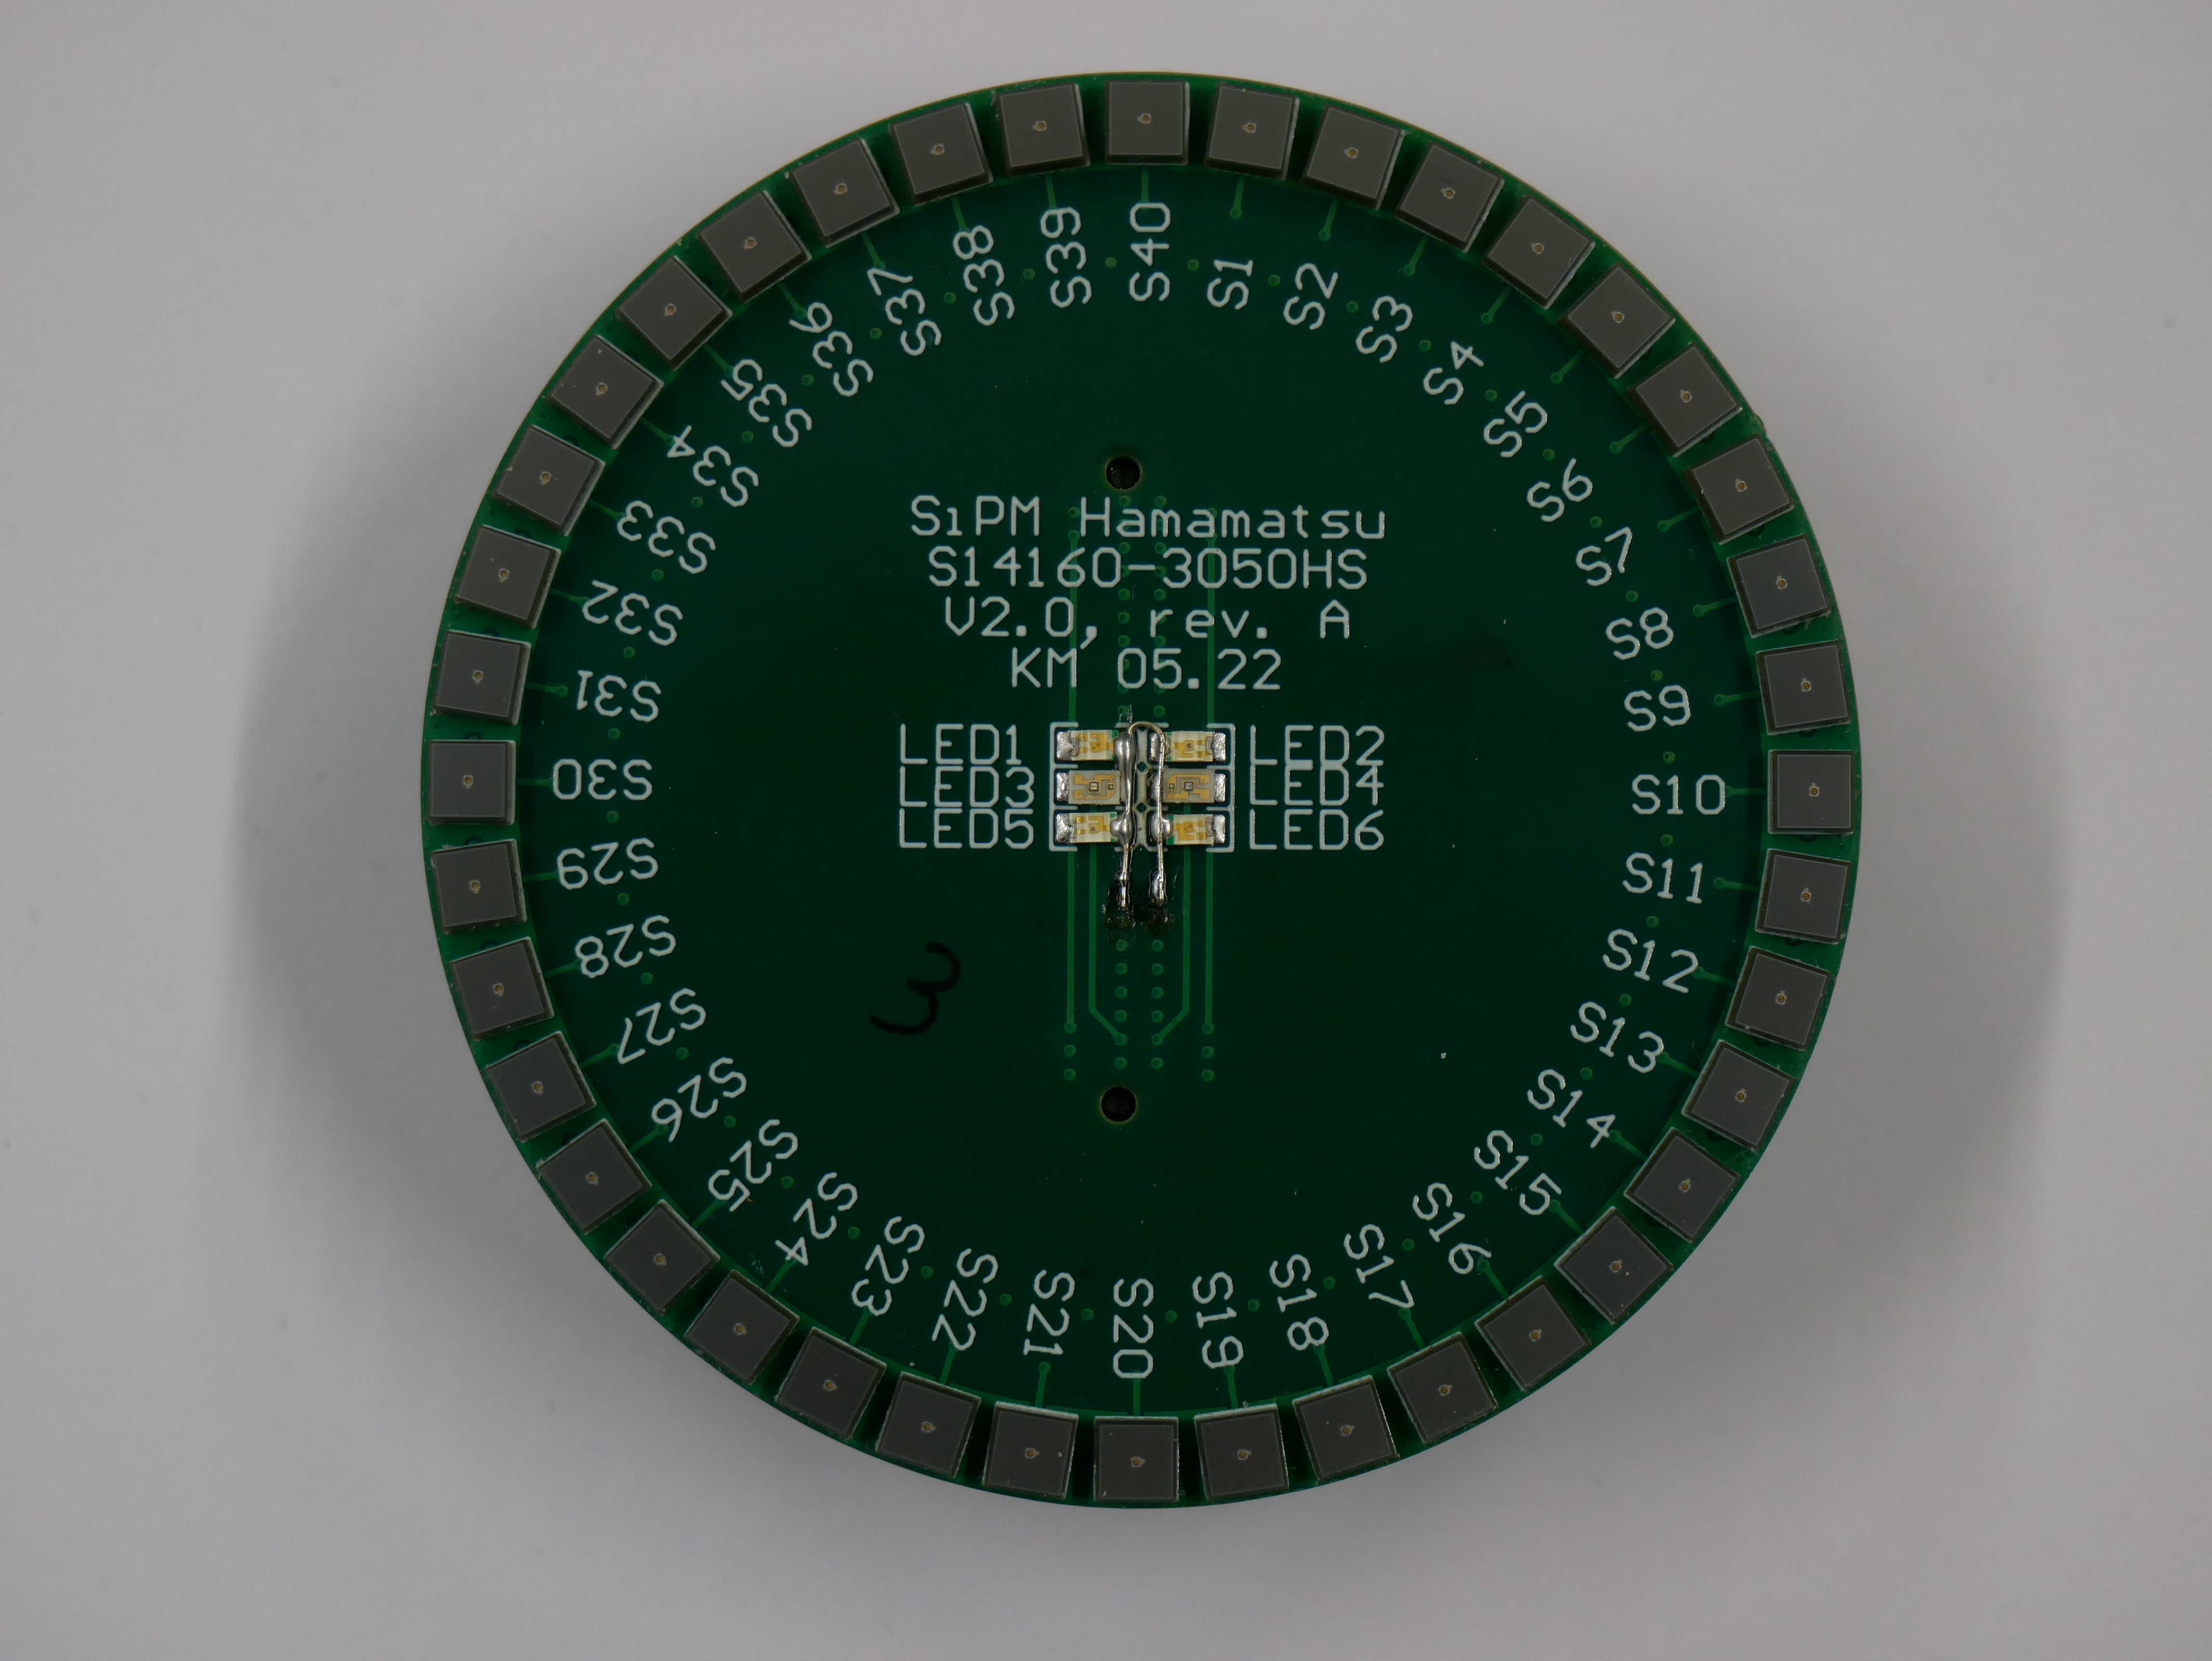
\includegraphics[width=.5\textwidth]{pictures/sipm_ham_pcb}
	\caption[\ac{pcb} with Hamamatsu \acp{sipm}]{One of the \acp{pcb} with Hamamatsu \acp{sipm} used for this work.}
	\label{fig:sipm_pcb}
\end{figure}

\section{Dark Box Setup}
To ensure a controlled evironment for the measurements, the \acp{sipm} were placed inside a dark box.
The inside of the box is covered in black aluminum foil made by Thorlabs with a reflectivity in the visible wavelength spectrum below \SI{5}{\percent} \cite{}.
An optical rail for fixing the \ac{sipm} board, a diffusor and the end of an optical fiber was placed in the box.
Via the optical fiber the light of a \SI{460}{\nano\meter} LED can be guided into the box.
The LED is inside of another light tight box.
It was build as part of the bachelor thesis of Alexander Bismark and is described there in more detail \cite{}.
Power can be supplied to the LED via a BNC connector on the light tight box.
In this thesis the Tektronix AFG was used to create voltage pulses with a width down to \SI{4}{\nano\second} with \SI{2.5}{\nano\second} rising and falling edges.
To eluminate all \acp{sipm} equaly a \textit{ED1-C50-MD} diffuser by Thorlabs was used.
A light beam hitting the diffusor perpendicular to its surface gets diffused in a circular shape with a \SI{50}{\degree} opening angle.
%The relative light intensity of the diffused light of a collimated \SI{488}{\nano\meter} laser beam measured by Thorlabs is shown in \autoref{fig:diffuser_dist} \cite{}.

Multiple BNC, SMA, and SMC feedthroughs were installed in the dark box to supply the \acp{sipm} and \ac{emusic} board with power and to transfer the output signals of the \ac{emusic} out of the box to a digitizer or oscilloscope.
Also a hole drilled to insert the optical fiber from the LED setup into the box and afterwards covered, to block light from entering through the hole.
A power supply was used for the high voltage supply of the \acp{sipm}.
If not otherwise specified, all measurements shown in this thesis were done with a high voltage of \SI{43}{\volt}.
To control the voltage the HP multimeter was used instead of the less precise voltage display of the power supply.
The \ac{emusic} board was powered by a \SI{8}{\volt} power supply.
For the digitization either a \ac{gandalf} or the Tektronix oscilloscope was used.

\autoref{fig:setup_sketch} shows a schmatic sketch of the setup inside and on the outside of the box.
A picture of the setup inside the box is shown in \autoref{fig:setup_box_pic}.
It includes the LED fiber, the diffuser, the \ac{sipm} and \ac{emusic} board with power and signal cables attached.
In the following the setup part with the \ac{gandalf} is described.
\begin{figure}
	\centering
	\includegraphics[]{}
	\caption[]{}
	\label{fig:setup_sketch}
\end{figure}
\begin{figure}
	\centering
	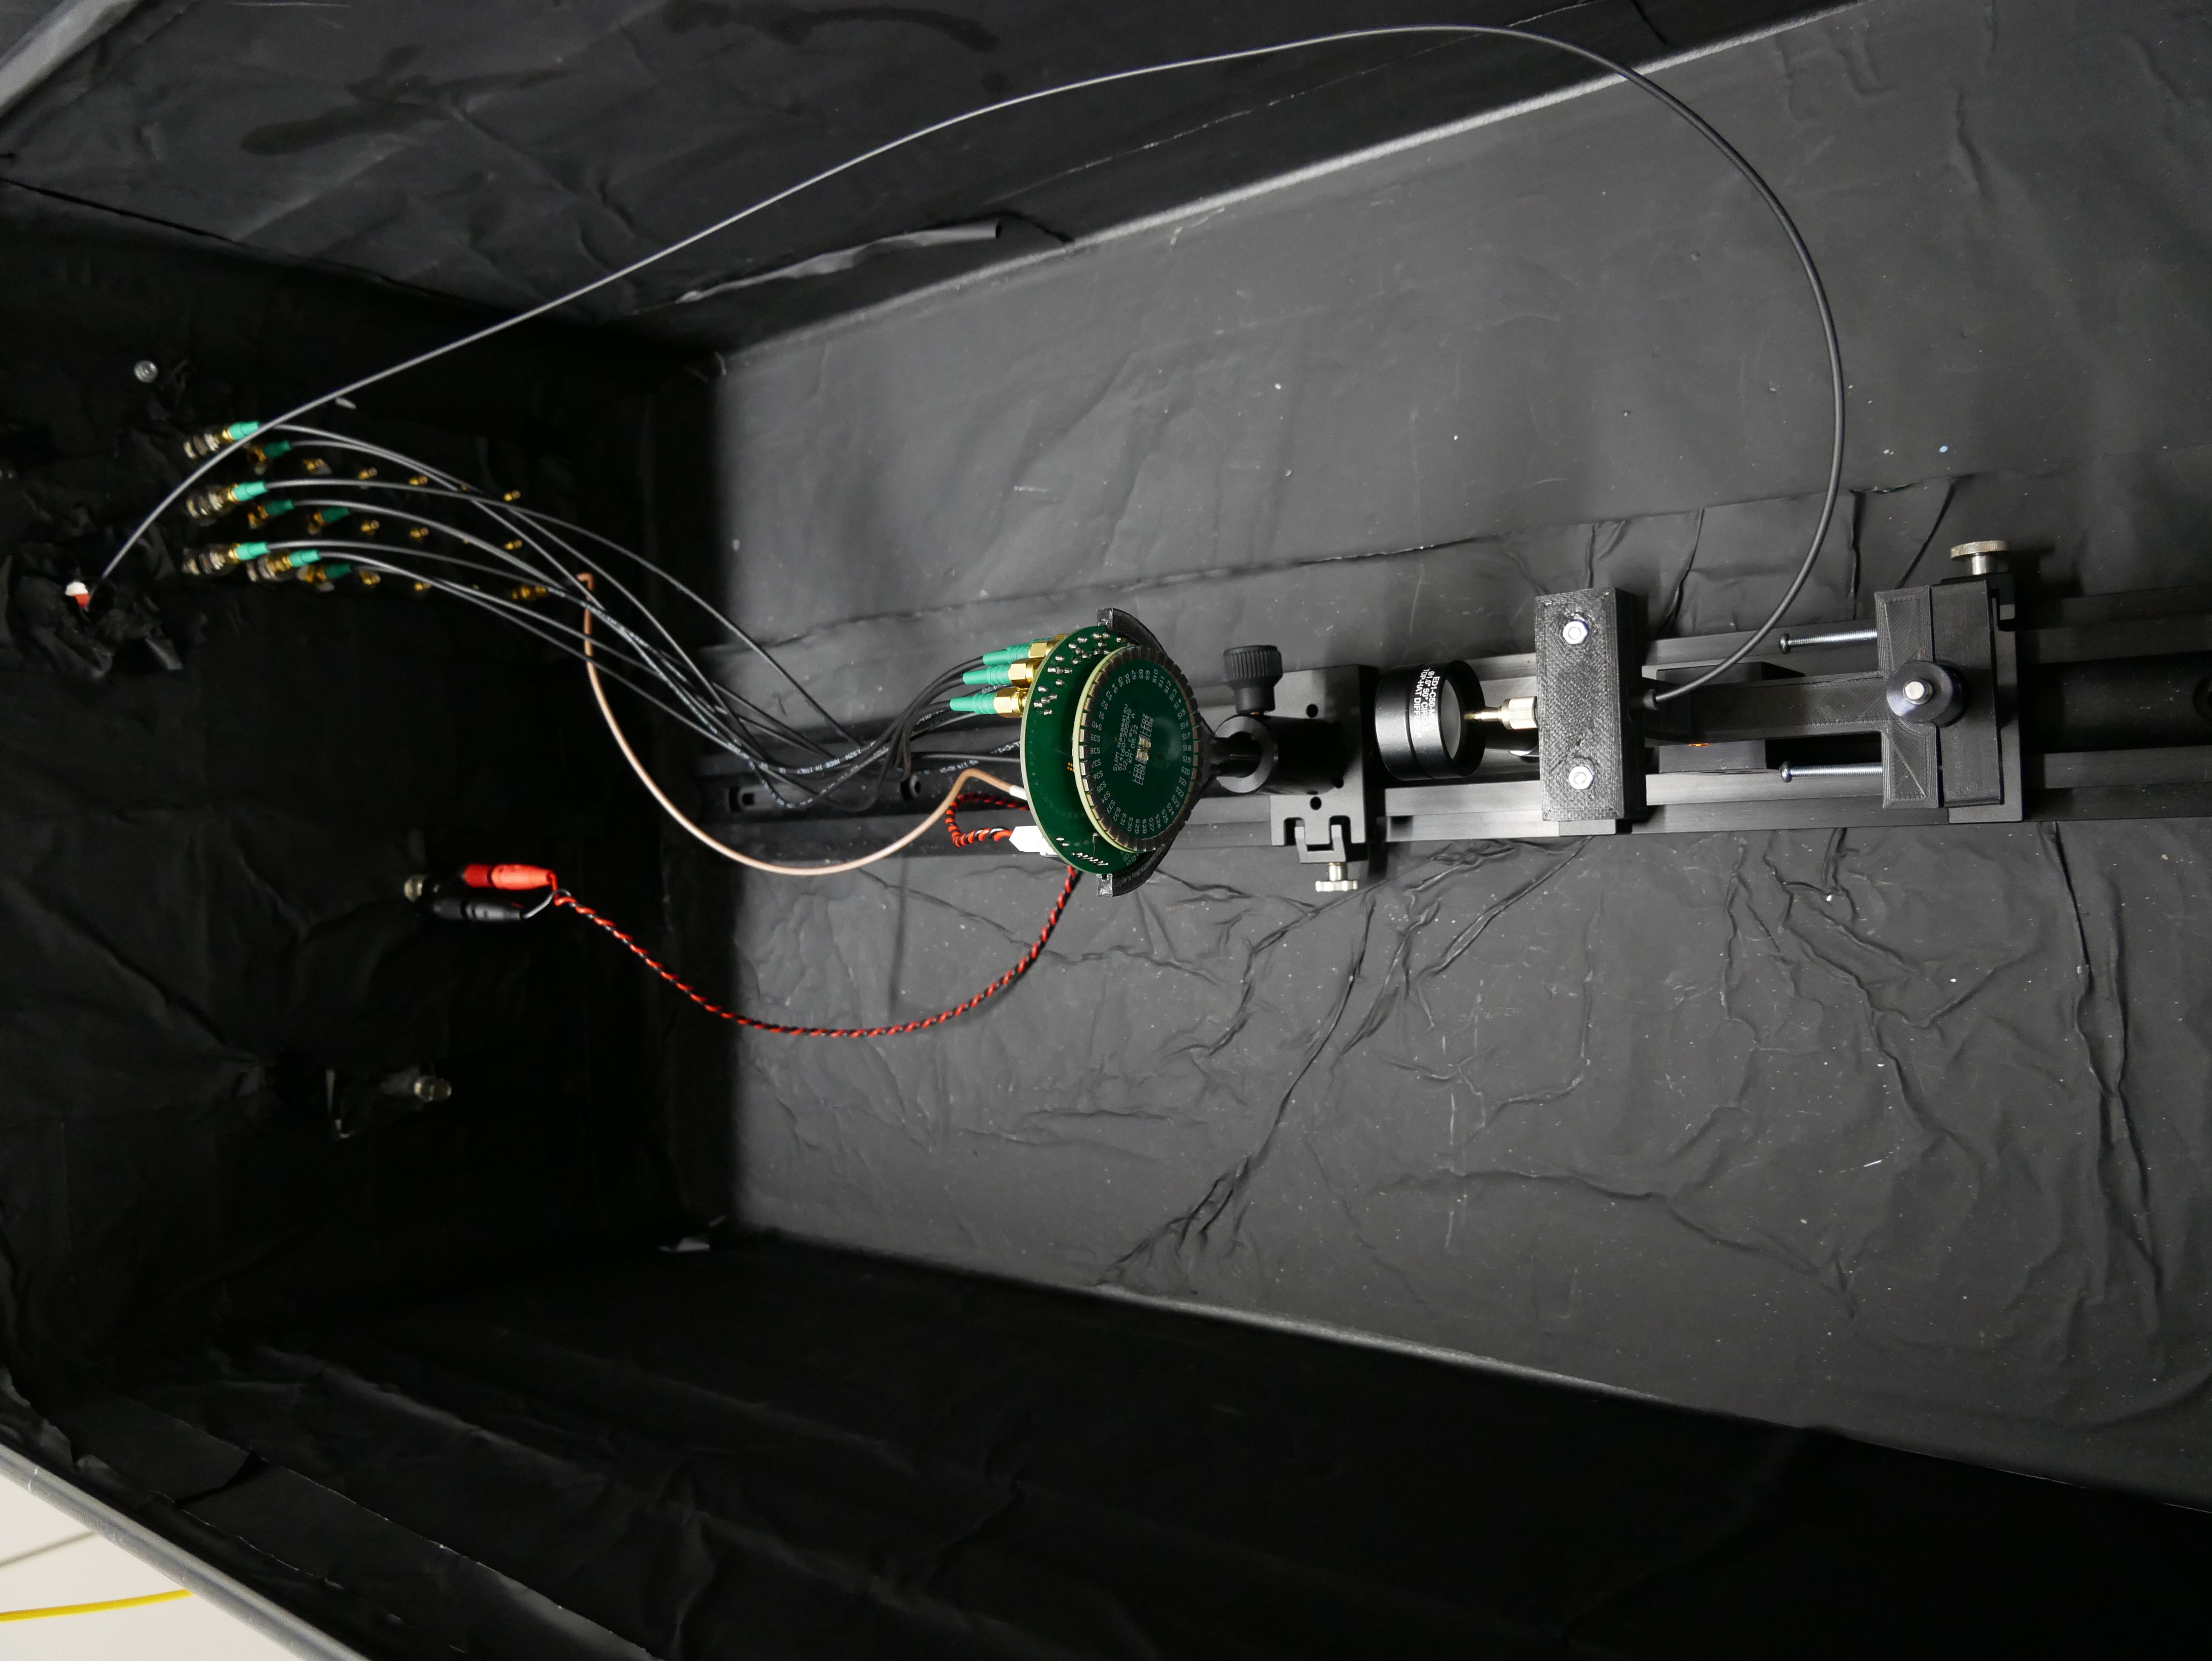
\includegraphics[width=0.5\textwidth]{pictures/setup_box_pic}
	\caption[Picture of the inside of the dark box.]{The inside of the dark box which was used for the test measurements. On the left is the end of the fiber from the LED setup mounted on the optical rail. Behind the fiber end is a diffuser by Thorlabs which diffuses the light in a circular distribution with an opening angle of \SI{50}{\degree}. After the diffuser is the \ac{pcb} with the \acp{sipm} placed. On its back is the \ac{emusic} board plugged in. The high voltage for the \acp{sipm} is supplied via the brownish cable, the power for the \ac{emusic} chip is supplied with the red and black cable and the signal outputs of the \ac{emusic} boards are connected with the feedthrough on the box via the black SMA cables.}
	\label{fig:setup_box_pic}
\end{figure}

\section{Gandalf}

For the operation of the One Cell Prototype sixteen channels need to be digitized, eight of each of the two \acp{wom}.
Therefore two \acp{gandalf} are required.
In order to save place and simplify the setup, the \acp{gandalf} are not operated in a VME crate but are each in a \ac{gandalf} portable.
It is a mobile case made exactly for such puroses where a whole crate is unconvinient.
A picture of a \ac{gandalf} portable is shown in \autoref{fig:gandalf_portable}.
Due to the usage of two \acp{gandalf} an external clock is required to ensure a syncronized sampling frequency and clock for time stamps.
As an external clock a copper GIMLI was chosen and used with a GIMLI testboard, shown in \autoref{fig:gimli_testboard}.
It has two slots for GMILIs, for each on data and one clock output and a power connector to supply it with \SI{5}{\volt}.
For the purpose of an external clock, only one of these slots and the corresponding clock output is used.
Via LEMO cables, the clock signal form the boards clock output pins is connected to the clock inputs of the \acp{gandalf}.
\begin{figure}
	\centering
	\begin{subfigure}[b]{.4\textwidth}
		\centering
		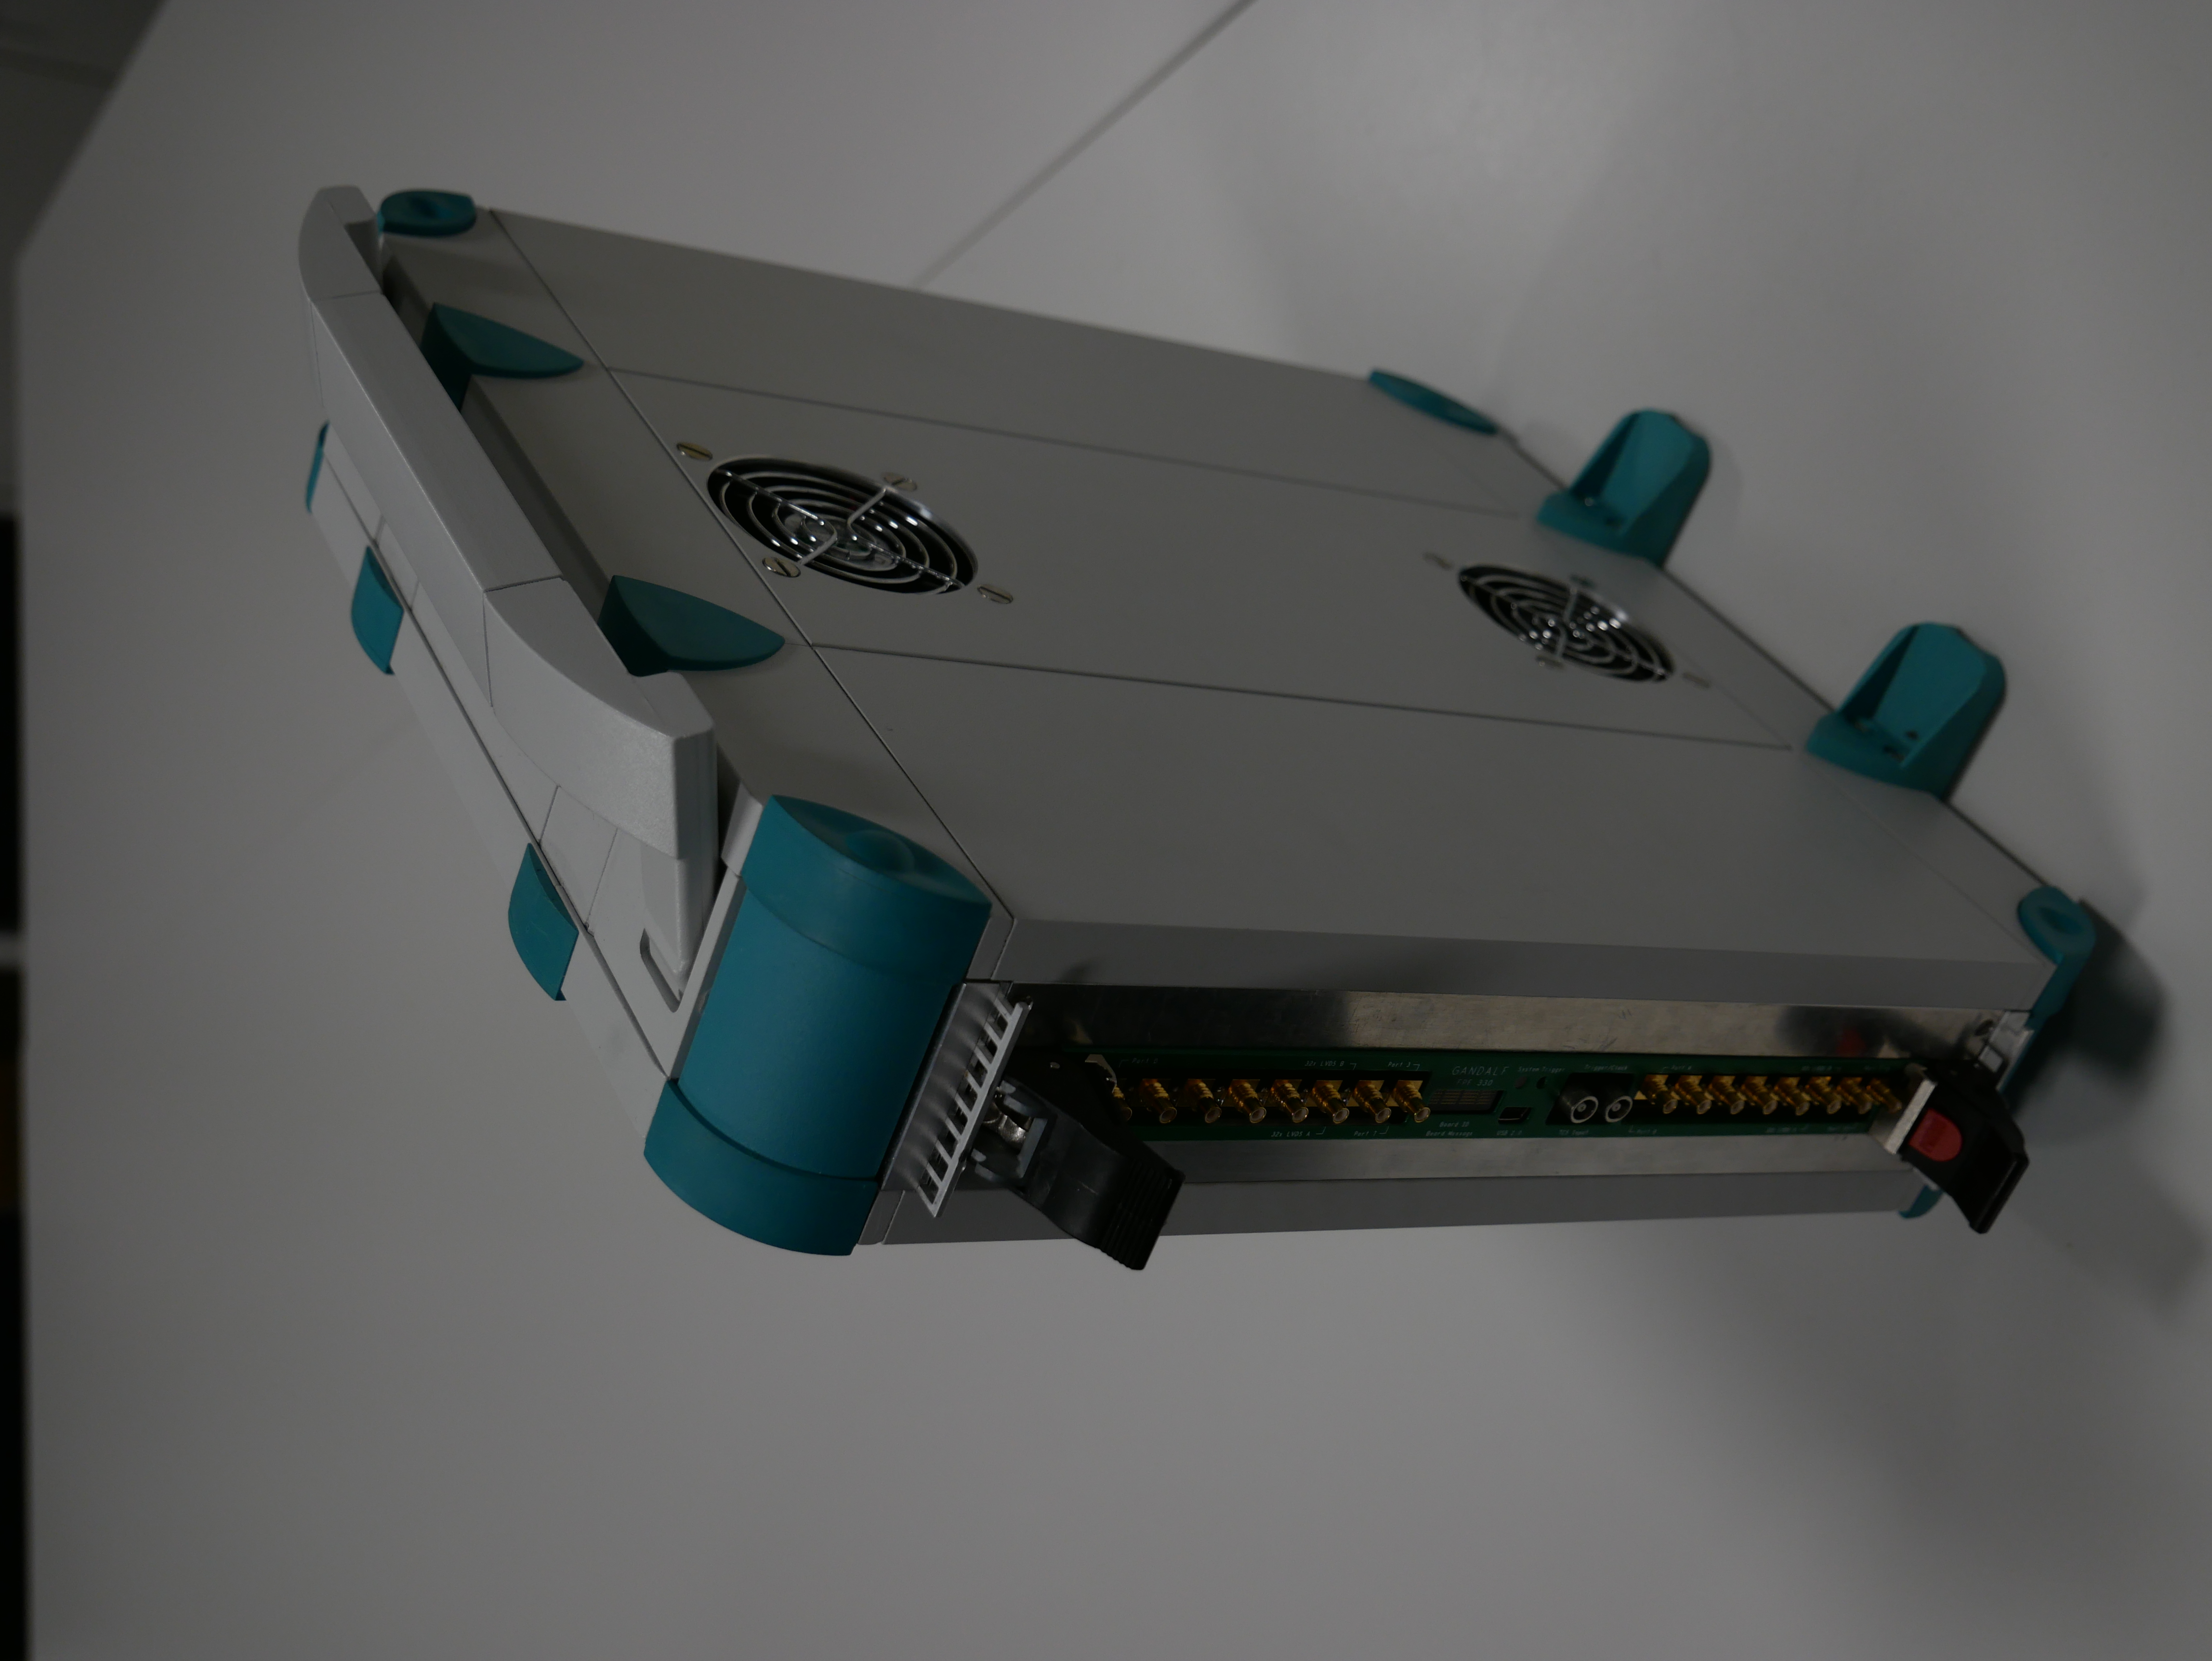
\includegraphics[width=1.\textwidth, angle=-90]{pictures/gandalf_portable} 
		\caption[A \ac{gandalf} portable equiped with a \ac{gandalf}.]{}
		\label{}
	\end{subfigure}
	\begin{subfigure}[b]{.55\textwidth}
		\centering
		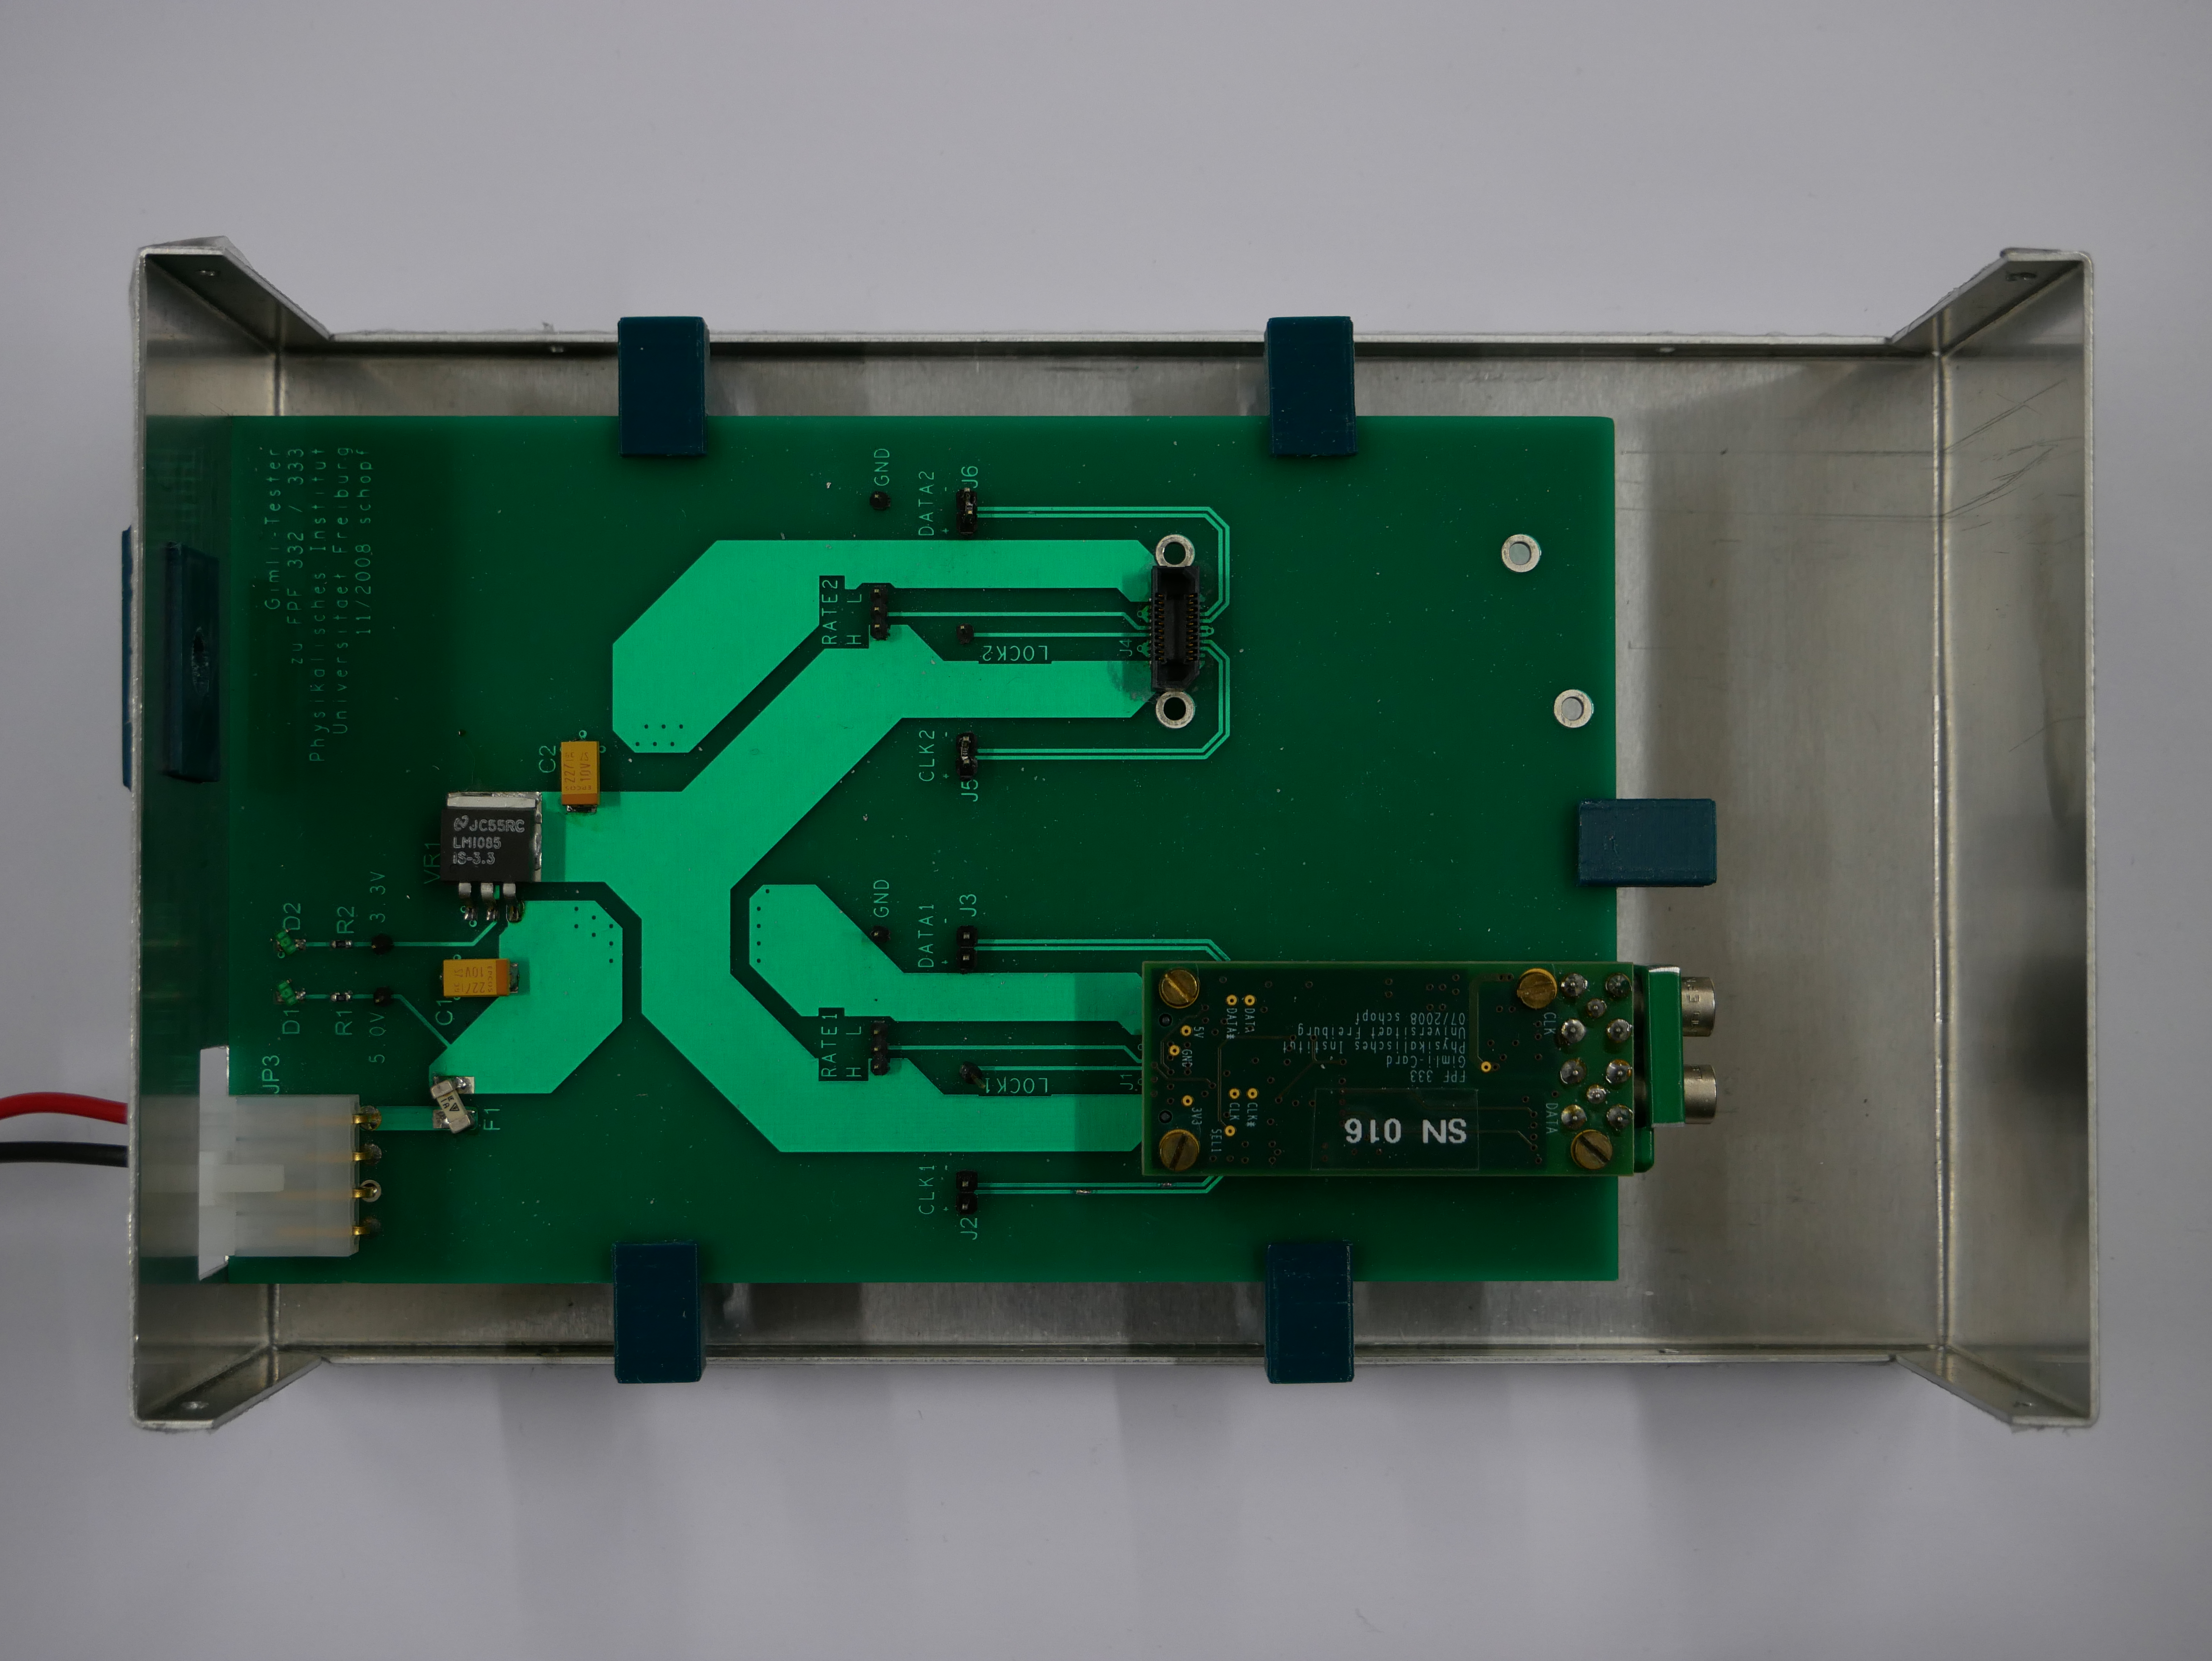
\includegraphics[width=1.\textwidth]{pictures/gimli_testboard}
		\caption[]{}
		\label{}
	\end{subfigure}
	\caption[]{A \ac{gandalf} portable equiped with a \ac{gandalf}. The GIMLI test board with a copper GIMLI}
	\label{}
\end{figure}
